\documentclass[11pt,a4paper]{article}
\usepackage[margin=0.75in,top=1.0in,bottom=0.9in,headheight=32pt]{geometry}
\usepackage{graphicx}
\usepackage{amsmath,amssymb}
\usepackage{listings}
\usepackage{fancyhdr}
\usepackage{lastpage}
\usepackage{xcolor}
\usepackage{caption}
\usepackage{subcaption}
\usepackage{float}
\usepackage{array}
\usepackage{hyperref}

% Document Palette matching Lycans AeroDesign branding
\definecolor{lycansnavy}{HTML}{0f2b46}
\definecolor{codebg}{HTML}{f8fafc}
\definecolor{codeframe}{HTML}{cbd5e1}
\definecolor{commentgreen}{HTML}{16a34a}
\definecolor{keywordblue}{HTML}{2563eb}
\definecolor{stringred}{HTML}{dc2626}
\definecolor{sectioncolor}{RGB}{27, 85, 131}
\definecolor{tableheader}{HTML}{cbd5e1}

\hypersetup{
    colorlinks=true,
    linkcolor=lycansnavy,
    urlcolor=lycansnavy,
    citecolor=lycansnavy
}

% Syntax highlighting configuration for code snippets
\lstset{
    backgroundcolor=\color{codebg},
    frame=single,
    rulecolor=\color{codeframe},
    basicstyle=\small\ttfamily,
    keywordstyle=\color{keywordblue}\bfseries,
    commentstyle=\color{commentgreen}\itshape,
    stringstyle=\color{stringred},
    breaklines=true,
    captionpos=b,
    keepspaces=true,
    showstringspaces=false
}

% Running Header and Footer Setup
\pagestyle{fancy}
\fancyhf{}
\lhead{\small\textbf{\color{lycansnavy} LYCANS AERODESIGN TEAM --- Trainee Assignment}}
\rhead{
\includegraphics[height=0.35in]{images/lycans_logo.png}}
\lfoot{\small Autonomous System and Software Integration}
\rfoot{\small Page \thepage\ of \pageref{LastPage}}
\renewcommand{\headrulewidth}{0.5pt}
\renewcommand{\footrulewidth}{0.5pt}

\begin{document}

% Header Block
\noindent
\begin{minipage}[c]{0.22\textwidth}

\includegraphics[width=1.3in]{images/lycans_logo.png}
\end{minipage}%
\hfill
\begin{minipage}[c]{0.75\textwidth}
{\LARGE \textbf{\color{lycansnavy} LYCANS AERODESIGN TEAM}}\\[4pt]
{\Large \textbf{Trainee Assignment Report}}\\[6pt]
\textbf{Name:} Trainee Member \\[2pt]
\textbf{Assignment:} Final Project \\[2pt]
\textbf{Date:} September 13, 2026\\[2pt]
\end{minipage}

\vspace{8pt}
\noindent\rule{\textwidth}{1pt}
\vspace{12pt}

\section{Overall System Architecture and Data Flow}

\subsection{System Overview}
A smartphone camera streams live video via IP Webcam to OpenCV for object detection. The \texttt{Perception Node} processes this and sends custom state frames to the \texttt{Decision Node}, which directs ArduPilot SITL maneuvers via \texttt{MAVROS}. 

\begin{center}
\textbf{Pipeline:} \texttt{Camera} $\rightarrow$ \texttt{OpenCV Processing} $\rightarrow$ \texttt{Custom ROS 2 Message} $\rightarrow$ \texttt{Decision Node} $\rightarrow$ \texttt{MAVROS} $\rightarrow$ \texttt{ArduPilot SITL}
\end{center}

\subsection{Object-Oriented Design}
We chose an Object-Oriented Programming (OOP) software architecture because it provides a highly structured and organized paradigm for team-based development. The codebase is modularized as follows:

\begin{itemize}
    \setlength\itemsep{0em}
    \item \textbf{\texttt{cv\_perception.py}:}
    \begin{itemize}
        \item \texttt{cameraStream}: Uses \texttt{get\_frame()} to return an active frame on each loop execution.
        \item \texttt{TargetDetector}: Applies \texttt{detect\_blue\_rectangle()} and \texttt{detect\_green\_circle()} for color masking and shape classification, returning command integers: \texttt{NONE} (0), \texttt{RTL} (1), or \texttt{LAND} (2).
        \item \texttt{ObstacleDetector}: Uses \texttt{detect\_red\_obj()} for masking. Computes object-to-frame area ratio to classify distance ranges (\texttt{TOOFAR}, \texttt{FAR}, \texttt{MID}, \texttt{NEAR}). Uses \texttt{obstacle\_direction()} to determine the X-coordinate column (\texttt{LEFT, CENTER, RIGHT}).
    \end{itemize}

    \item \textbf{\texttt{perception\_node.py}:}
    \begin{itemize}
        \item \texttt{PackMsg} \& \texttt{PerceptionNode}: Uses \texttt{packvars()} to pack output values into a ROS 2 custom \texttt{Detection.msg} and publishes it onto the \texttt{vision/detection\_cmd} topic.
    \end{itemize}

    \item \textbf{\texttt{decision\_manager.py}:}
    \begin{itemize}
        \item \texttt{DetectionInput} \& \texttt{Decision}: Encapsulates raw data (command, obstacle presence, distance) and chosen flight actions.
        \item \texttt{DecisionManager}: Evaluates \texttt{DetectionInput}. Returns avoidance decisions for hazards, or \texttt{RTL}/\texttt{LAND} decisions for targets. Uses \texttt{update\_confirmed\_mode()} to prevent redundant commands.
    \end{itemize}

    \item \textbf{\texttt{mavros\_interface.py} \& \texttt{constants.py}:}
    \begin{itemize}
        \item \texttt{MavrosInterface}: Executes \texttt{request\_mode()} and \texttt{send\_avoidance()} to dispatch repositioning commands.
        \item \texttt{constants.py}: Centralized configuration (\texttt{COMMAND\_RTL = 1}, \texttt{FAR\_OFFSET = 43.0\,m}).
    \end{itemize}
\end{itemize}

\begin{figure}[H]
    \centering
    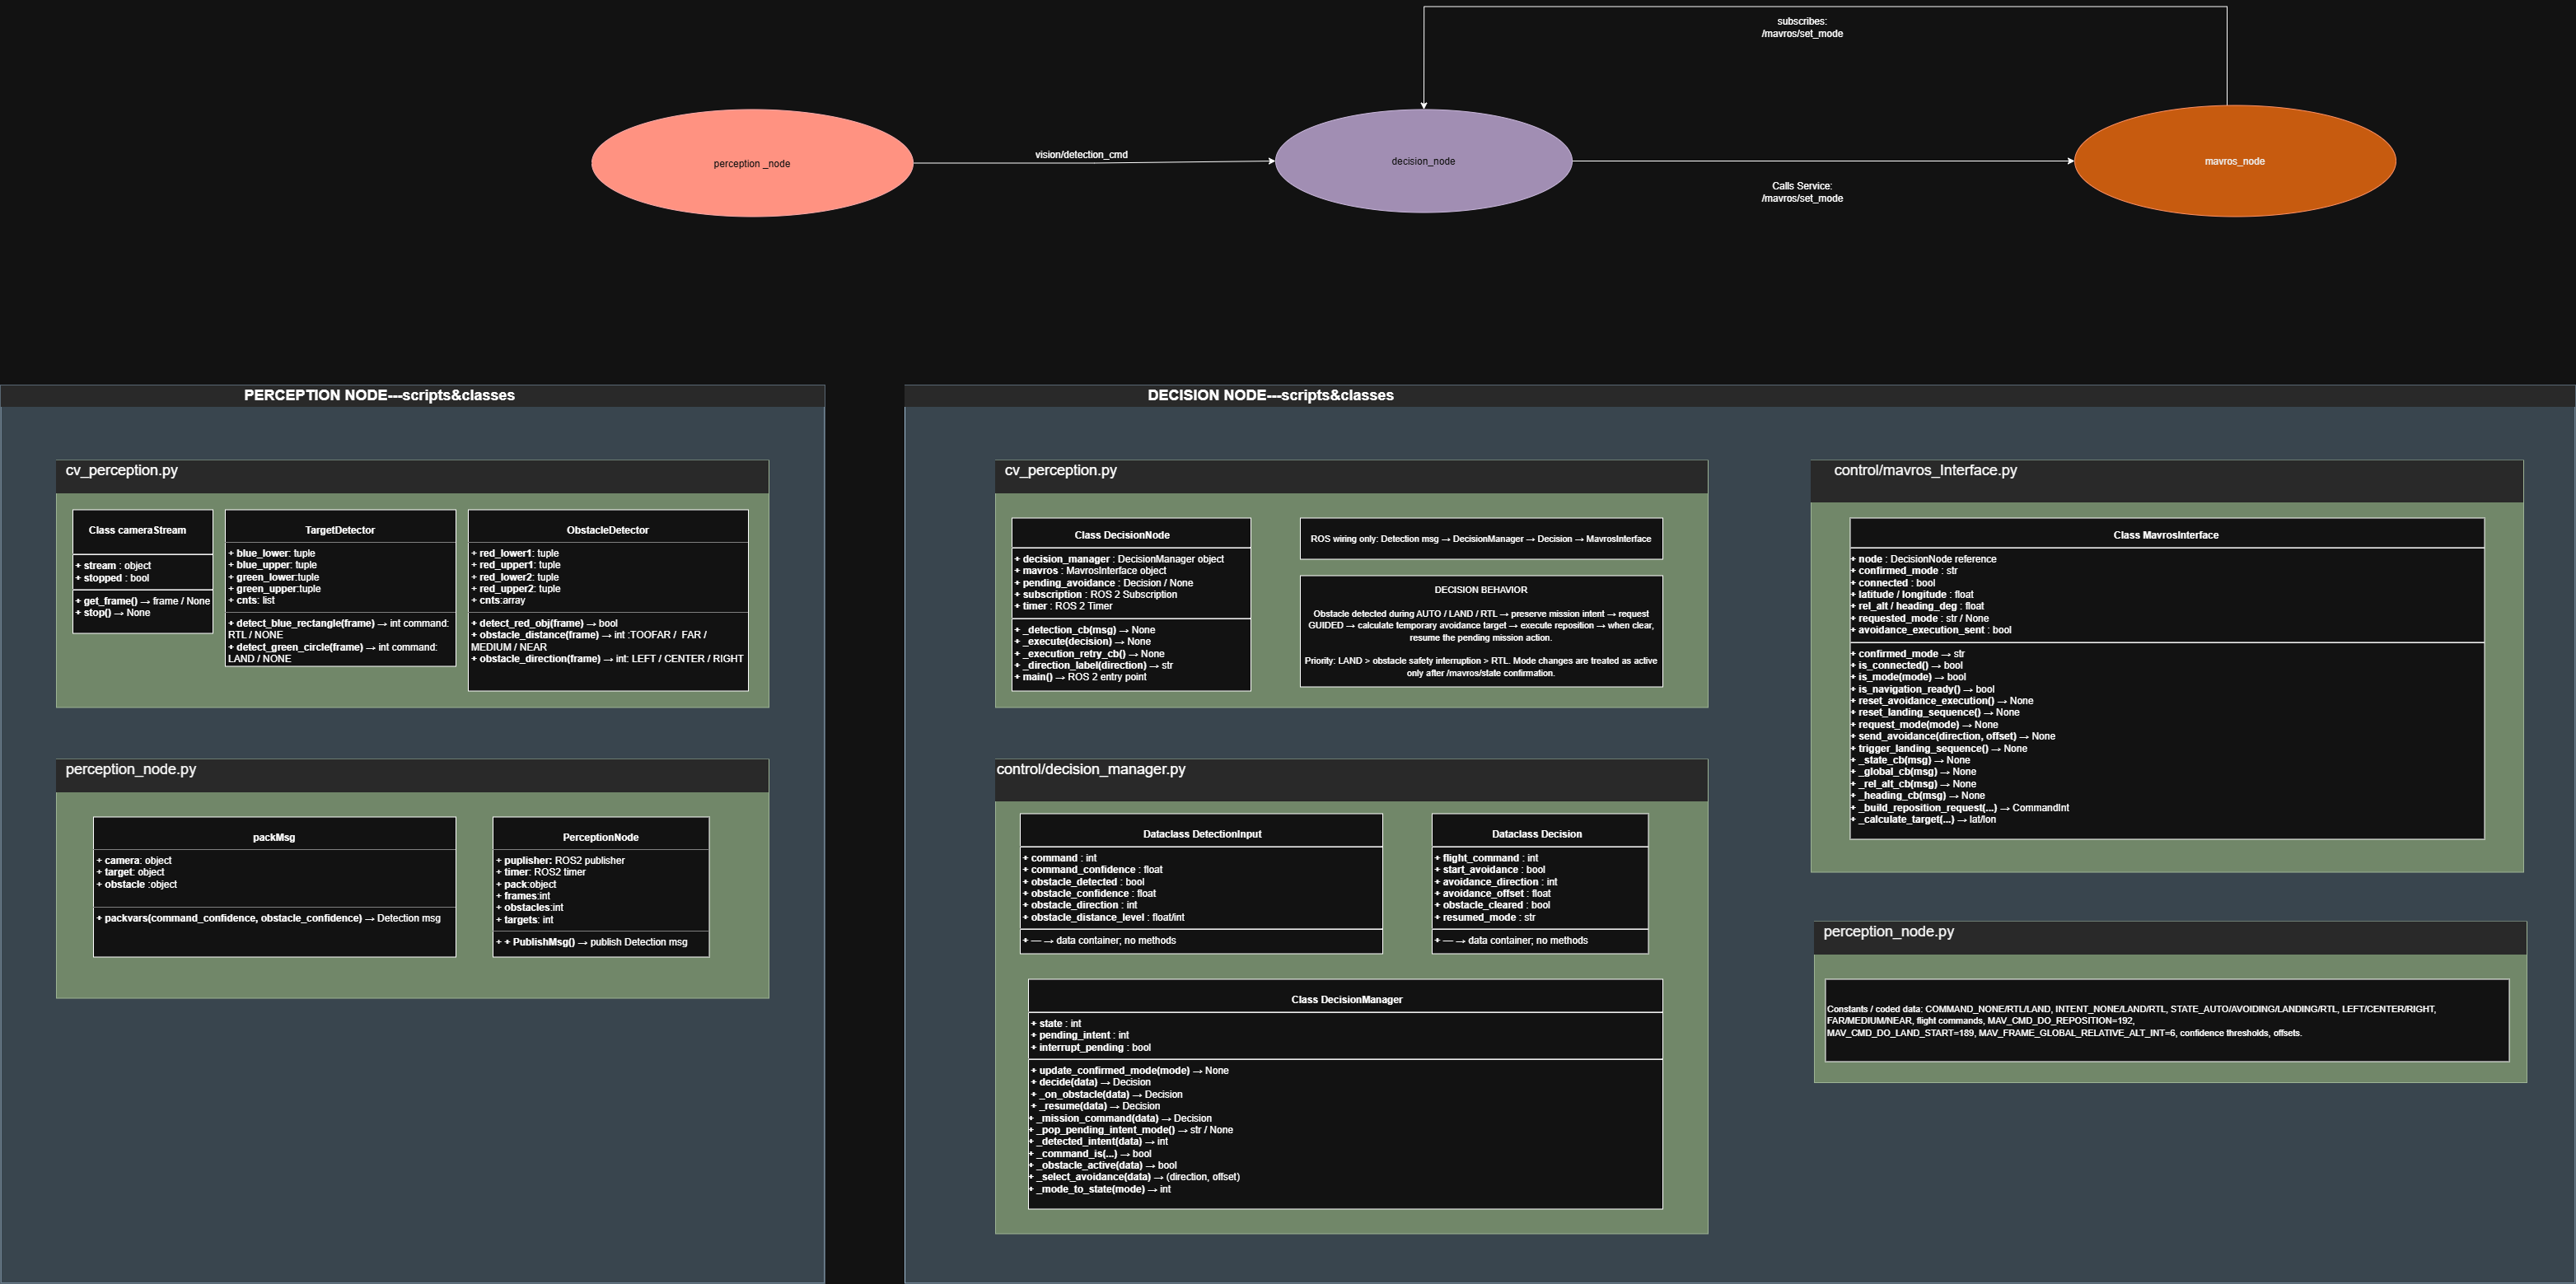
\includegraphics[width=0.85\textwidth]{images/oop_diagram1.drawio.png}
    \caption{Object-Oriented Architecture and ROS 2 Node Interaction Diagram.}
    \label{fig:oop_diagram}
\end{figure}

\section{ROS 2 Node Structure, Topics, and MAVROS}

\subsection{Custom Interfaces \& Node Architecture}
The system consists of \texttt{perception\_node} (Publisher) and \texttt{decision\_node} (Subscriber). Communication relies on \texttt{Detection.msg} in the \texttt{pada\_interfaces} package:

\begin{lstlisting}[language=bash, caption={Custom ROS 2 Message Definition (Detection.msg)}]
int8 command
float32 command_confidence
bool obstacle_detected
float32 obstacle_confidence
int8 obstacle_direction
int8 obstacle_distance
\end{lstlisting}

\subsection{MAVROS Integration}
The \texttt{Decision Node} communicates with ArduPilot SITL using MAVROS:
\begin{itemize}
    \setlength\itemsep{0em}
    \item \textbf{Flight Mode Switches:} Calls \texttt{/mavros/set\_mode} to command \texttt{RTL}, \texttt{LAND}, \texttt{GUIDED}, and \texttt{AUTO}.
    \item \textbf{Obstacle Avoidance:} Invokes \texttt{/mavros/cmd/command\_int} with \texttt{MAV\_CMD\_DO\_REPOSITION} (192), translating avoidance offsets into updated global GPS targets.
\end{itemize}

\begin{figure}[H]
    \centering
    \includegraphics[width=0.7\textwidth]{images/ros2_graph.png}
    \caption{ROS 2 Node Computational Graph (\texttt{rqt\_graph}).}
\end{figure}

\section{Visual Perception and Mode Mapping}

\subsection{Perception Strategy \& Shape Classification}
Frames are converted to HSV via $Frame_{HSV} = \texttt{cv2.cvtColor}(Frame_{BGR}, \text{HSV})$ for robust thresholding via \texttt{cv2.inRange()}. Contours are extracted (\texttt{cv2.findContours}) and approximated:
\begin{equation}
\epsilon = 0.02 \times P_{\text{contour}}, \quad \text{Vertices} = |\texttt{cv2.approxPolyDP}(\text{contour}, \epsilon, \text{True})|
\end{equation}
\textbf{4 Vertices:} Quadrilateral (Rectangle). \textbf{$>8$ Vertices:} Circle.

\subsection{Mode Mapping Definition}
\begin{table}[H]
\caption{Visual Perception Command to Flight Mode Mapping}
\centering
\begin{tabular}{@{}p{1.2in}p{1.8in}p{1.4in}p{1.8in}@{}}
\hline
\rowcolor{tableheader}
\textbf{Target Color} & \textbf{Geometry} & \textbf{Command Code} & \textbf{Triggered Flight Action} \\ \hline
Blue & Rectangle (4 vertices) & \texttt{COMMAND\_RTL} (1) & Return-To-Launch (\texttt{RTL}) \\
Green & Circle ($>8$ vertices) & \texttt{COMMAND\_LAND} (2) & Precision Landing (\texttt{LAND}) \\
Red & Any shape ($A > 500\text{ px}$) & Hazard Flag & Guided Obstacle Avoidance \\ \hline
\end{tabular}
\end{table}

\section{Decision-Making and Obstacle Avoidance}

\subsection{Obstacle Distance \& Direction Calculation}
Distance relies on the area ratio: $A_{\text{ratio}} = (A_{\text{object}} / A_{\text{frame}}) \times 100\%$.
\begin{equation}
\text{Distance Level} = 
\begin{cases}
\text{\texttt{TOOFAR} (2)}, & A_{\text{ratio}} < 5\% \\
\text{\texttt{FAR} (1)}, & 5\% \le A_{\text{ratio}} < 10\% \\
\text{\texttt{MID} (0)}, & 10\% \le A_{\text{ratio}} < 15\% \\
\text{\texttt{NEAR} (-1)}, & A_{\text{ratio}} \ge 15\%
\end{cases}
\end{equation}

Direction utilizes spatial moments ($c_x = M_{10} / M_{00}$) divided into three partitions:
\textbf{\texttt{LEFT} (-1):} $0 \le c_x < \frac{1}{3} W$, \textbf{\texttt{CENTER} (0):} $\frac{1}{3} W \le c_x < \frac{2}{3} W$, \textbf{\texttt{RIGHT} (1):} $\frac{2}{3} W \le c_x \le W$.

\subsection{Avoidance \& Recovery Engine}
When hazard data is received, the \texttt{DecisionManager} interrupts the mission for \texttt{GUIDED} mode. \texttt{MavrosInterface} calculates an offset GPS coordinate (e.g., $+43.0\,\text{m}$) and dispatches the repositioning. Once the obstacle clears, it requests \texttt{AUTO} to seamlessly resume the waypoint mission.

\section{Error Handling and Efficiency}
\begin{itemize}
    \setlength\itemsep{0em}
    \item \textbf{Noise Filtering:} Background clutter is mitigated by strictly ignoring contours where Area $< 500$ px (\texttt{if cv2.contourArea(c) > 500:}).
    \item \textbf{Stream Reliability:} Latency crashes are prevented by verifying frame integrity (\texttt{if frame is None: return}) before processing.
    \item \textbf{Computational Efficiency:} To prevent processing lag, contours are sorted by area, and evaluation is restricted to the top 5 largest shapes (\texttt{[:5]}).
\end{itemize}

\section{Evidence from the SITL Demonstration}
A full mission validation was conducted in ArduPilot SITL. The aircraft executed an \texttt{AUTO} waypoint mission, encountered a simulated red obstacle requiring dynamic path alteration, and subsequently processed visual command targets to execute \texttt{RTL} and \texttt{LAND} mode transitions.

\begin{figure}[H]
    \centering
    \includegraphics[width=0.65\textwidth]{images/Ardupilot.png}
    \caption{SITL flight execution and telemetry tracking.}
\end{figure}

\section*{\textcolor{sectioncolor}{Bonus Task 1 — SITL Log Debugging Challenge}}
\addcontentsline{toc}{section}{Bonus Task 1 — SITL Log Debugging Challenge}

The provided \texttt{BROKEN\_LOGS.BIN} contains multiple deliberately injected faults. The analysis below distinguishes handled non-critical anomalies from the primary cause of control loss.

\begin{table}[H]
\centering
\small
\begin{tabular}{|p{0.18\textwidth}|p{0.18\textwidth}|p{0.56\textwidth}|}
\hline
\rowcolor{tableheader}
\textbf{Finding} & \textbf{Time} & \textbf{Evidence / Interpretation} \\
\hline
Airspeed Anomaly & 48.005--155.025~s & \texttt{SIM\_ARSPD\_FAIL} produces abnormal airspeed ($\sim$345~m/s). The failure is detected/disabled by ArduPilot and navigation falls back to GPS; not the final crash cause. \\
\hline
RC Failure & 114.745~s & \texttt{SIM\_RC\_FAIL}=1 causes throttle failsafe. The aircraft safely switches to Auto at 119.805~s, demonstrating proper protective response. \\
\hline
Battery Drop & 69.685 / 95.384~s & \texttt{SIM\_BATT\_VOLTAGE} reduced to 9.5~V and 8.5~V. No battery-failsafe action is recorded; does not explain the loss of control. \\
\hline
\textbf{Elevator Reversal (Root Cause)} & \textbf{156.205~s} & \textbf{\texttt{SERVO2\_REVERSED}=1 reverses the elevator response (\texttt{SERVO2\_FUNCTION}=19). Measured pitch diverges rapidly to $-80^\circ$ before impact at 27.48~m/s.} \\
\hline
\end{tabular}
\end{table}

\begin{figure}[H]
    \centering
    \begin{minipage}[b]{0.45\textwidth}
        \centering
        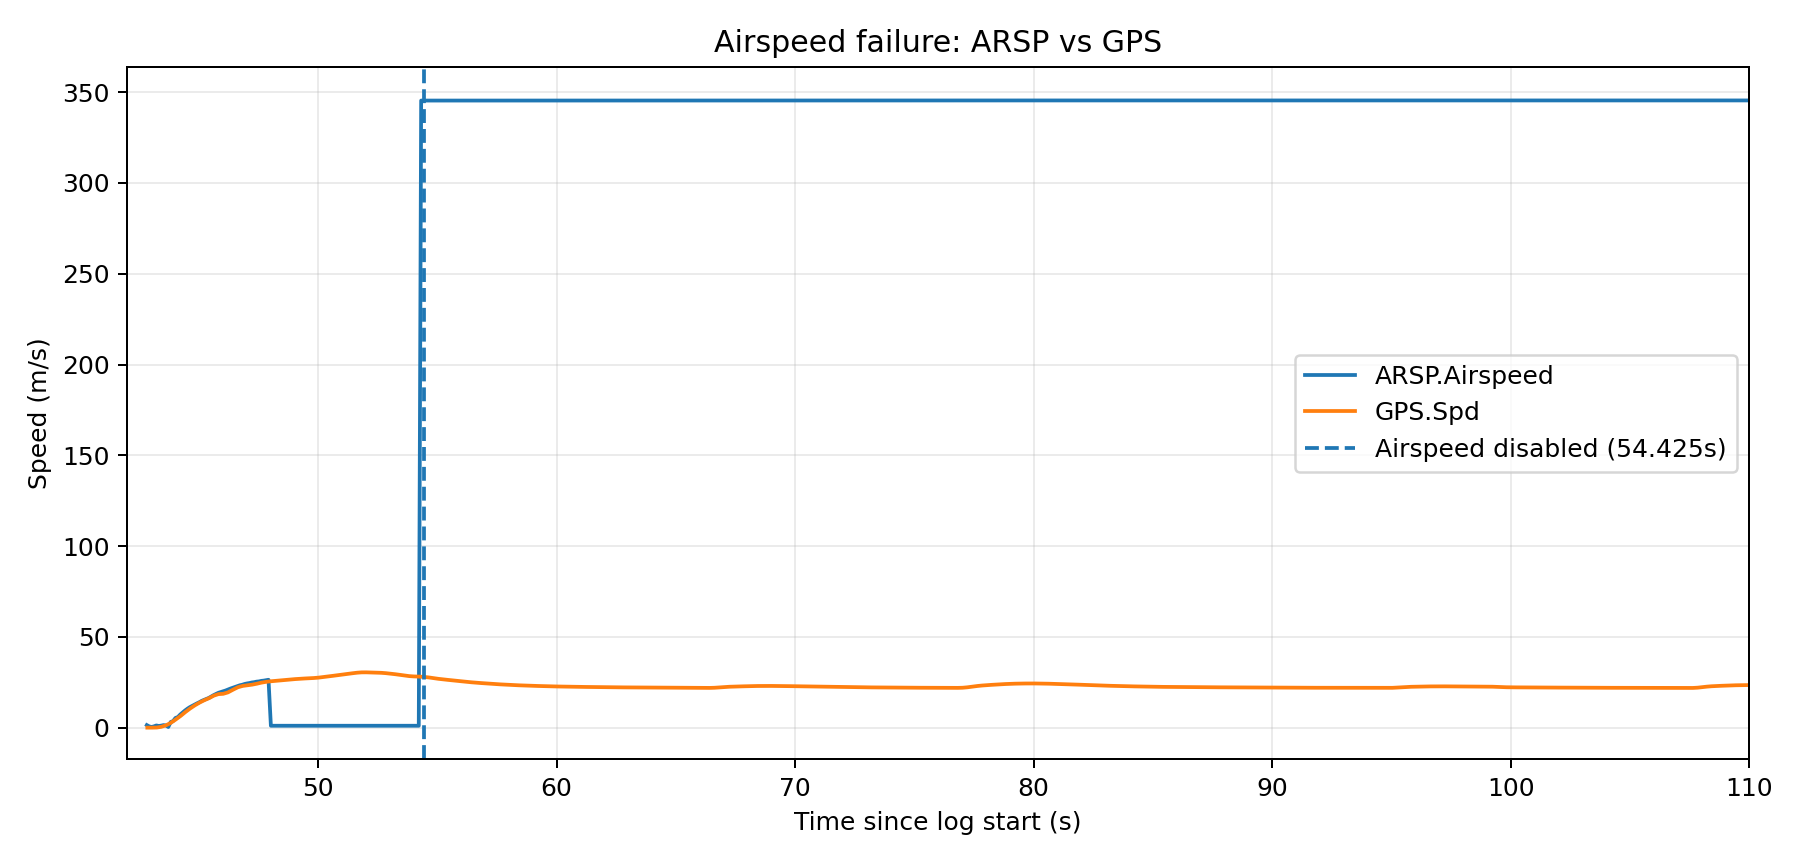
\includegraphics[width=\textwidth]{images/image1.png}
    \end{minipage}
    \hfill
    \begin{minipage}[b]{0.45\textwidth}
        \centering
        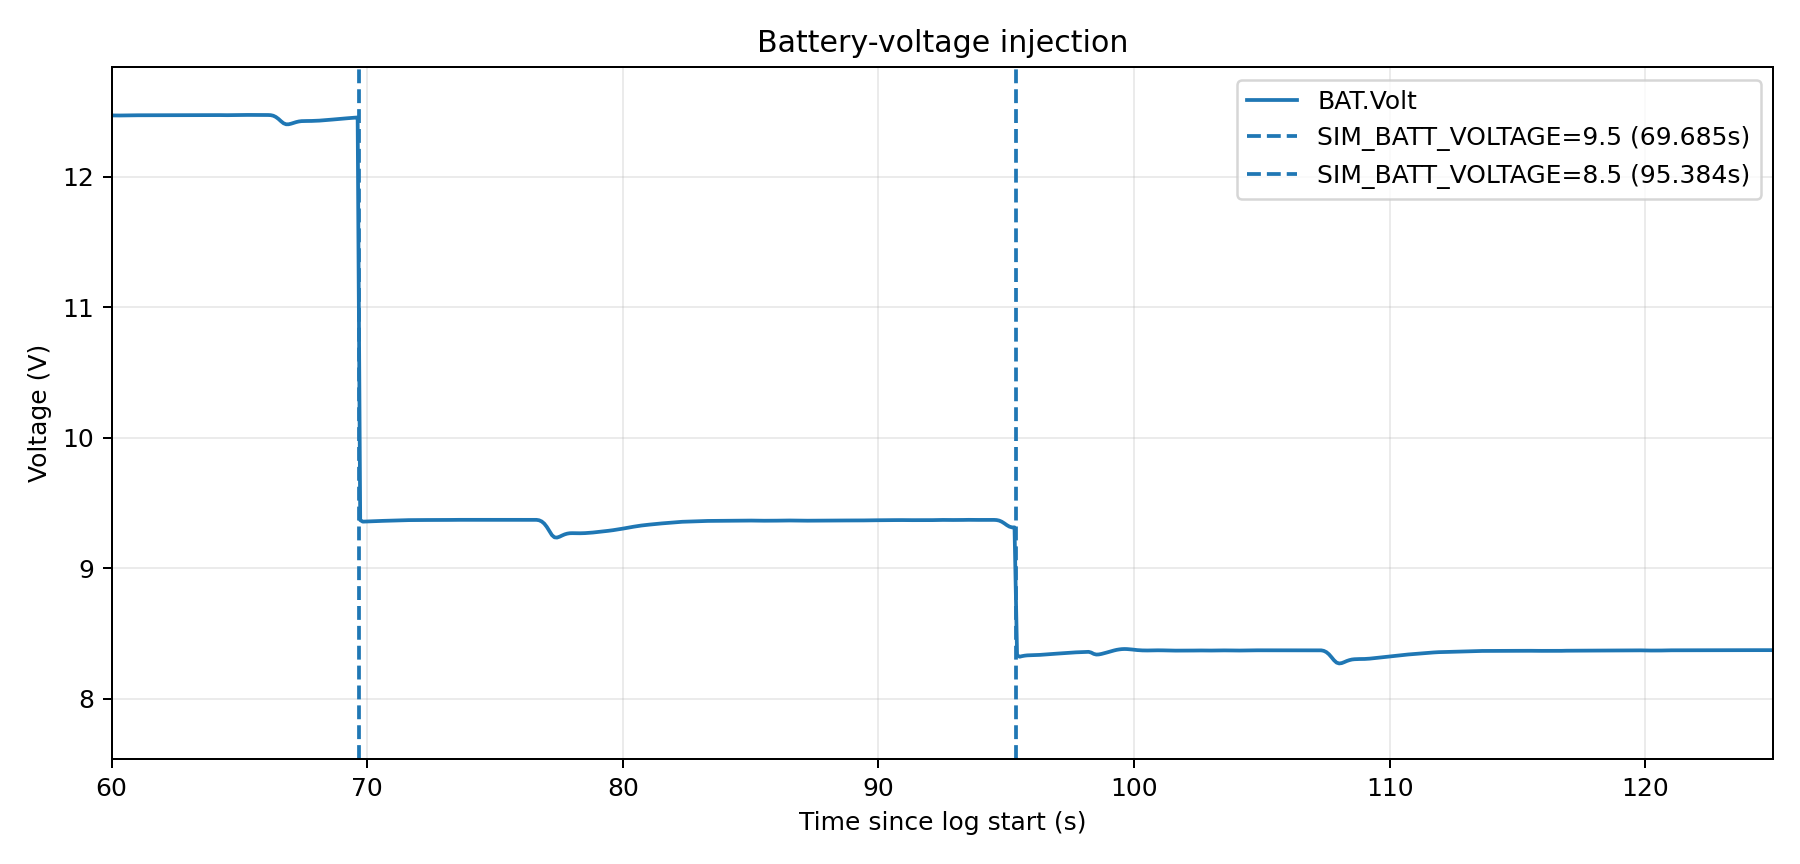
\includegraphics[width=\textwidth]{images/image2.png}
    \end{minipage}
    \vspace{0.2cm}
    
    \begin{minipage}[b]{0.45\textwidth}
        \centering
        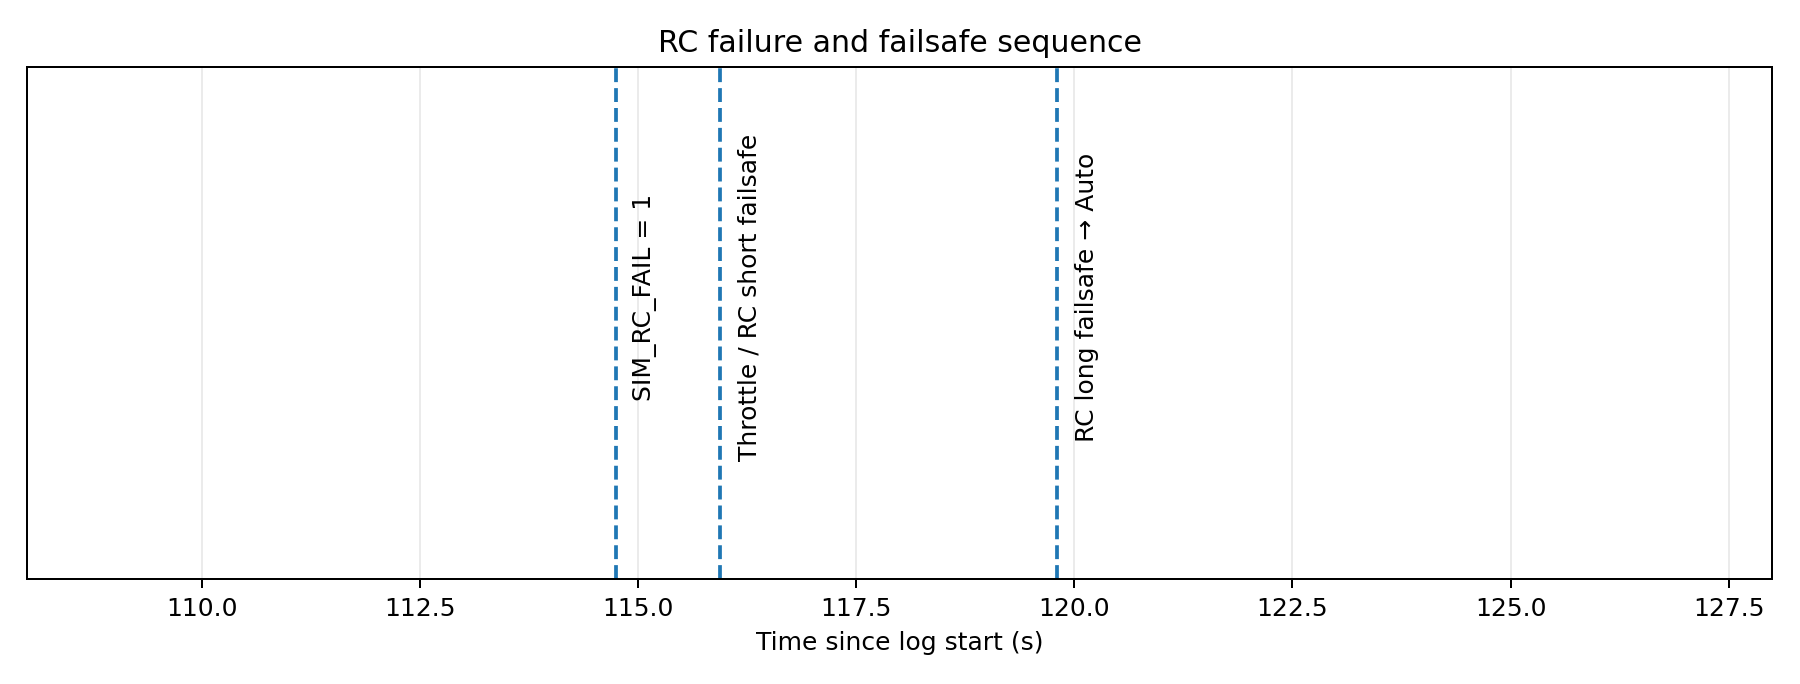
\includegraphics[width=\textwidth]{images/image3.png}
    \end{minipage}
    \hfill
    \begin{minipage}[b]{0.45\textwidth}
        \centering
        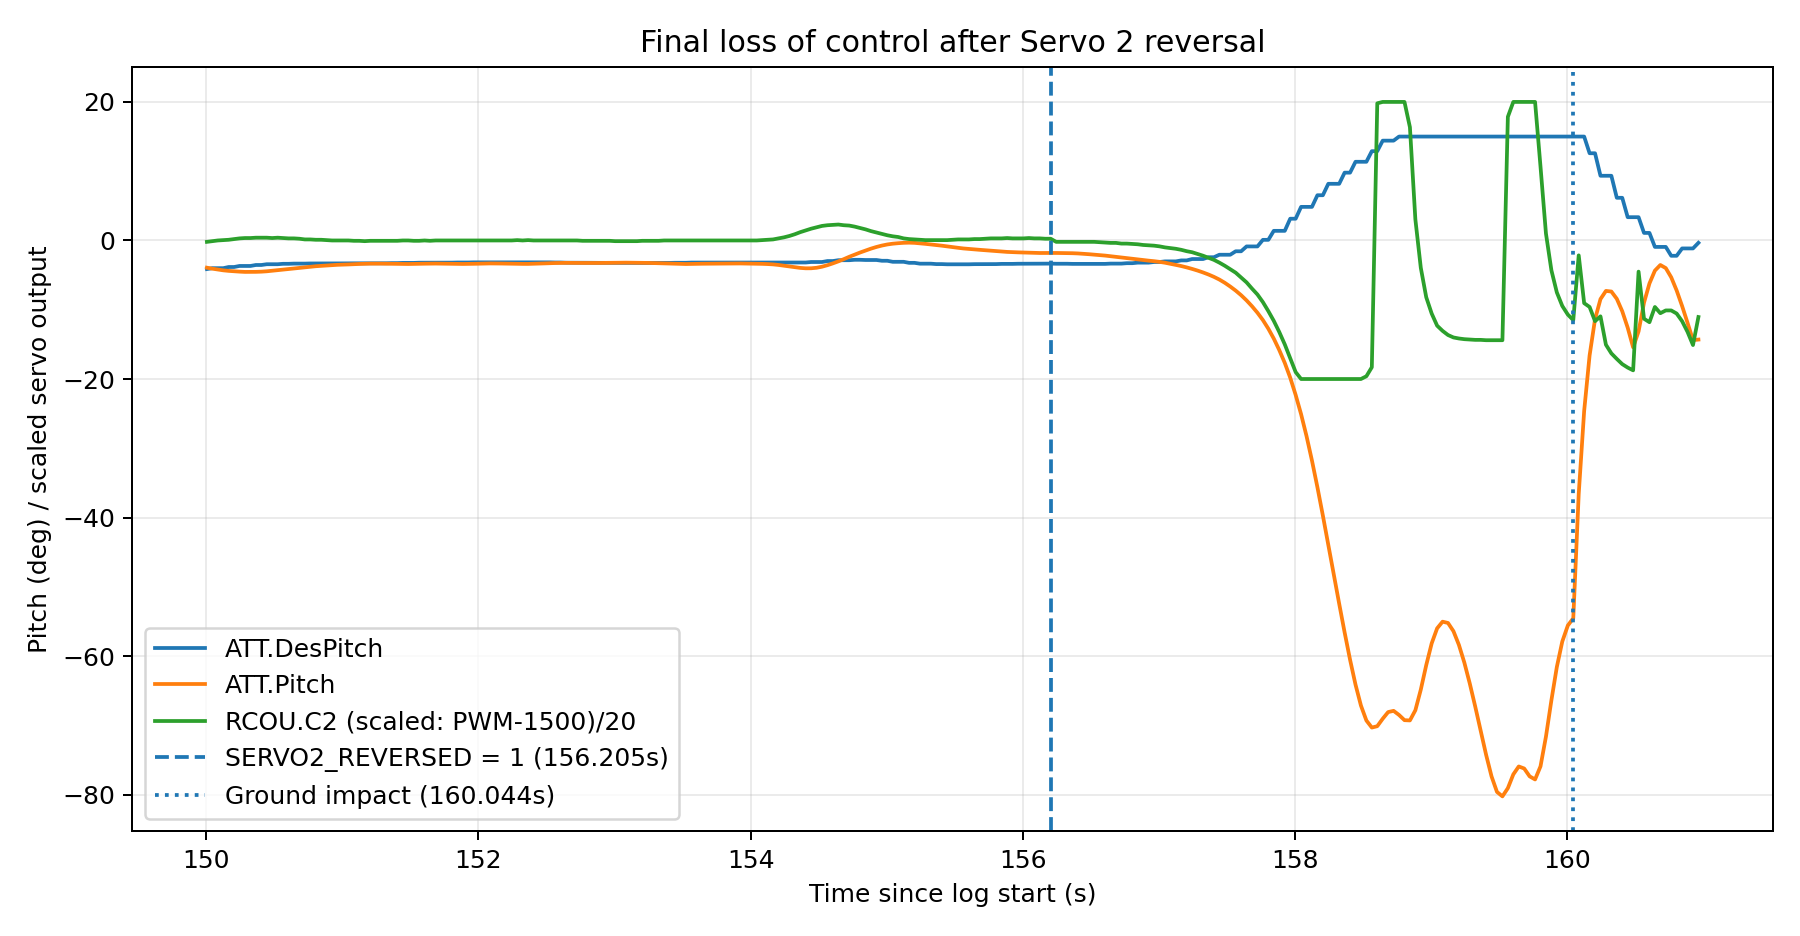
\includegraphics[width=\textwidth]{images/image4.png}
    \end{minipage}
    \caption*{\footnotesize \textcolor{darkgray}{Flight-log evidence plots demonstrating sensor anomalies and pitch divergence.}}
\end{figure}

\subsection*{\textcolor{sectioncolor}{Corrective Actions}}
\begin{enumerate}
    \setlength\itemsep{0em}
    \item Restore \texttt{SERVO2\_REVERSED = 0} to correct elevator deflection direction, and verify \texttt{SERVO2\_FUNCTION = 19} in SITL pre-flight checks.
    \item Reset \texttt{SIM\_RC\_FAIL = 0} and verify the intended RC-failsafe settings.
    \item Reset \texttt{SIM\_ARSPD\_FAIL = 0} and \texttt{SIM\_ARSPD\_FAILP = 0} to restore primary airspeed sensor fusion.
    \item Restore nominal battery voltage telemetry and configure appropriate low-voltage failsafes.
\end{enumerate}

\section*{\textcolor{sectioncolor}{Final Software Assessment}}
The integrated system supports all required operations: normal \texttt{AUTO} waypoint flight, \texttt{GUIDED} avoidance and mission recovery, and \texttt{RTL/LAND} visual command processing. The architecture remains modular, relying on safety mechanisms such as 10-frame visual confirmation, 20\%/5\% obstacle hysteresis, and pending-intent preservation.

\end{document}